\subsubsection{Temperature Encoding} \label{sec:theory-approach-methodology-temperature-encoding}

\begin{figure}[t]
	\centering
	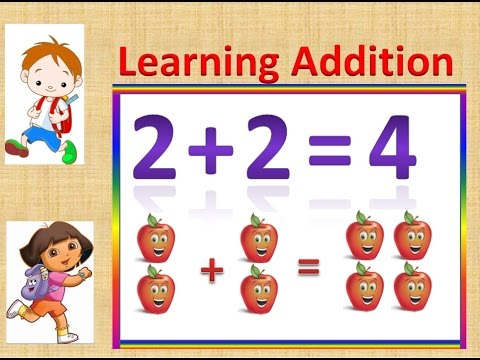
\includegraphics[max width=0.5\textwidth]{children-addition}
	\caption{An image that uses pictograms of apples to teach small children how to perform addition. Here children are taught to add 2 + 2 by counting two apples and then counting another two apples to make four apples\cite{learning_2015}.}
	\label{fig:children-addition}
\end{figure}

In the previous section, we discussed two methods by which symbols can guide our neural networks to develop good representations. We believe a neural network model can discover functions such as carry forward, especially if a clear symbol is present that allows the model to learn a consistent representation of the input handwritten digits. However, discovering an algorithm that generalizes to unseen digits is not straightforward since the model will not have learned this unseen sequence of digits before. In this section we describe the third and final stage of our theory development that we believe will overcome this difficulty.

In the beginning of this chapter we gave an example of how children learn to perform arithmetic using familiar objects. Figure \ref{fig:children-addition} depicts how this process works. Learners are presented a problem of adding 2 + 2 to produce 4. The problem is presented using traditional mathematical symbols such as the digits and the plus operator. Below the digits, pictures of apples are also used to convey the meaning of the digits and mathematical operator. Children are taught that performing the 2 + 2 operation is like counting two apples and then counting another two apples to obtain four apples.

Over time, human learners gain the ability to map the images of these familiar objects to the digits, especially to the quantities represented by the digits, and that performing arithmetic operations on the digits depends on the ability of the learner to successfully make this mapping. Children then later develop the ability to translate digits into quantities without the need for symbols of the digits. They are also able to perform these arithmetic operations without having to memorize every possible combination of digits, instead relying on the general solution they acquired with the aid of this symbolic knowledge.

In order to establish the analogy between learning with symbols in humans and learning with symbols in artificial neural networks we must show that we can develop a learning system that is able to learn:
\begin{itemize}
	\item the ordinal relationships between the digit operands, also known as successorship,
	\item the quantity or size each digit represents, and
	\item the function of the operator.
\end{itemize}
Human learners are able to use the knowledge transferred through the use of the symbols described above to capture all three aspects. The clear symbols provided to our neural network models should in turn be able to also represent these aspects\cite{wiki:Elementary_arithmetic}. 

When contrasting the symbols used by children to learn arithmetic and our proposed symbols, we notice that our one-hot vector representation lacks the ability to convey these aspects. The apples in Figure \ref{fig:children-addition} for example clearly indicate to a child the quantity represented by the digits. It also allows the learner to compare quantities and determine an ordinal relationship between the quantities and their respective digits. The one-hot vector symbols however do not have that ability.

\begin{figure}[t]
	\centering
	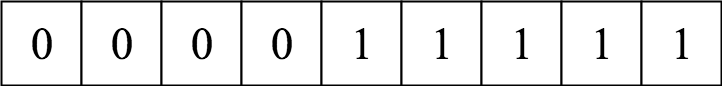
\includegraphics[max width=\textwidth]{temperature-encoding}
	\caption{The number 5 encoded in a vector using temperature encoding.}
	\label{fig:temperature-encoding}
\end{figure}

To overcome this problem, we need a better representation for our symbols. We therefore propose encoding the symbols using temperature encoding. A temperature encoded integer is a vector of binary values that has as many values sequentially set to one, starting from the right, as the integer being represented. Figure \ref{fig:temperature-encoding} is a depiction of the digit 5 encoded using temperature encoding. This type of encoding was chosen because, besides providing a clear vector representation for the digit, it also conveys the quantity of the digit that allows the model to capture the ordinal relationship between the digits. We expect that this will work better than one-hot encoding for learning an algorithm that can generalize to previously unseen digit combinations.
